%\documentclass[letterpaper, 10 pt, conference]{ieeeconf}  % Comment this line out
                                                          % if you need a4paper
\documentclass[a4paper, 10pt, conference]{ieeeconf}      % Use this line for a4
                                                          % paper

%\IEEEoverridecommandlockouts                              % This command is only
                                                          % needed if you want to
                                                          % use the \thanks command
%\overrideIEEEmargins
% See the \addtolength command later in the file to balance the column lengths
% on the last page of the document


\usepackage[utf8]{inputenc}
\usepackage[T1]{fontenc}

% The following packages can be found on http:\\www.ctan.org
%\usepackage{graphics} % for pdf, bitmapped graphics files
%\usepackage{epsfig} % for postscript graphics files
%\usepackage{mathptmx} % assumes new font selection scheme installed
%\usepackage{mathptmx} % assumes new font selection scheme installed
\usepackage{amsmath} % assumes amsmath package installed
%\usepackage{amssymb}  % assumes amsmath package installed
\usepackage{graphicx}
\usepackage[font={small,it}]{caption}
\usepackage{algorithm}
\usepackage{algorithmicx}
\usepackage{algpseudocode}
\renewcommand{\figurename}{Fig.}
\renewcommand{\tablename}{Tab.}
\renewcommand{\algorithmicrequire}{\textbf{Input:}}
%\renewcommand{\algorithmicensure}{\textbf{Output:}}

\addtolength{\oddsidemargin}{-.375in}
\addtolength{\evensidemargin}{-.375in}
\addtolength{\textwidth}{0.75in}
\addtolength{\topmargin}{-.475in}
\addtolength{\textheight}{1.2in}

\algdef{SE}[SUBALG]{Indent}{EndIndent}{}{\algorithmicend\ }%
\algtext*{Indent}
\algtext*{EndIndent}

%\renewcommand{\abstractname}{Resumo}
%\renewcommand\refname{Refer\^encias}

\title{\LARGE \bf
Mega Exercise 2: Delaunay triangulation
}

\author{Vitor Mazal Krauss}

\begin{document}

\maketitle
\thispagestyle{empty}
\pagestyle{empty}


%%%%%%%%%%%%%%%%%%%%%%%%%%%%%%%%%%%%%%%%%%%%%%%%%%%%%%%%%%%%%%%%%%%%%%%%%%%%%%%%
\begin{abstract}
In this project, I start by implementing the incremental algorithm for obtaining a triangulation of a 2D point set.
Following, I implement an edge flipping algorithm to obtain a Delaunay triangulation from a given triangulation.
Finally, I present a simple example of the usage of Delaunay triangulation for surface reconstruction.
\end{abstract}

%%%%%%%%%%%%%%%%%%%%%%%%%%%%%%%%%%%%%%%%%%%%%%%%%%%%%%%%%%%%%%%%%%%%%%%%%%%%%%%%

\section{Introduction}
The purpose of this project is to implement the incremental algorithm for obtaining a triangulation of a 2D point set and, followingly, to implement an algorithm to obtain a Delaunay triangulation from the incremental triangulation. 
A detailed description of the incremental algorithms are given in \cite{dcg, cg13}.
The algorithm for obtaining a Delaunay triangulation from any given one is better described in \cite{cg13}, in which it is referred to as the Lawson Flip Algorithm.
Finally, for a practical application of the Delaunay triangulation, I present an example of using a Delaunay triangulation for surface reconstruction, and compare the results with the reconstruction obtained from the incremental triangulation. 
The implementations were made in the C++ language, using the \textit{Standard Template Library} for general-purpose algorithms and data structures.
The \textit{GLM} library was used for the mathematical parts.
At last, I use the \textit{libigl} library for displaying the obtained triangulations and surfaces.

\subsection{Incremental Triangulation}
The Incremental Triangulation algorithm can be implemented with a simple addition to the Incremental Algorithm for Convex Hulls.
In the convex hull incremental algorithm, at each step, we must check which edges of the previously constructed hull are ``visible'' to the point being added.
By sorting the points based on their $x$-coordinate, we can provide a simple way to check visibility: it suffices to check whether the three points(the two vertices of the edge and the new point) are in clockwise order.
In order to obtain a triangulation from the incremental algorithm, we simply add a new step: for every visible edge, we add a new triangle, made up of the two vertices of that edge and the point being added.
Note, however, that we still have to keep track of the hull points of the given point set: at each step, we should only add triangles with vertices on the current hull.
If we were to add triangles with interior points, we would have edges crossing and, thus, violating the definition of triangulation.
Effectively, this means that by the end of the algorithm, it will have computed both the convex hull and a triangulation for the point set.
Since many triangles can share one same vertex, it is more efficient, memory-wise, to work in terms of indices, instead of the points itself.
Said this, in short, the algorithm I implemented keeps track of the indices of the hull points, which is updated at every step, and whenever a point is added, we add triangles(represented by $3$-uple of indices), formed from the new point and the visible edges.
Note that this means that the Incremental Triangulation algorithm has the same complexity as the Convex Hull Incremental Algorithm, which is $\mathcal{O}(n^2)$.

\subsection{Lawson Flip Algorithm}
This algorithm is described in \cite{cg13} as the Lawson Flip Algorithm.
This algorithm makes use of \textit{empty circle property} \cite{dcg, cg13} which effectively caracterizes Delaunay triangulations: for any triangle in a Delaunay triangulaion, the three vertices of this triangle describe a unique circle that circumscribes them. 
These points satisfy the empty circle property if no other point of this point set is inside this circumscribing circle.
For each internal edge of the triangulation there are exactly two triangles which share that edge.
Consider two triangles $\triangle p_1p_2p_3$ and $\triangle p_2p_3p_4$, sharing the edge $e = \overline{p_{2}p_{3}}$.
The edge $e$ satisfies the empty circle property if $p_4$ is not inside the circle that circumscribes $\triangle p_1p_2p_3$ or, equivalently, if $p_1$ is outside the circle that circumscribes $\triangle p_2p_3p_4$.
If the edge does satisfy the property, nothing has to be done.
On the other hand, if the edge does not satisfy the empty circle property, we must perform an edge flip: flipping the edge $e = \overline{p_{2}p_{3}}$ means substituting the triangles $\triangle p_1p_2p_3$ and $\triangle p_2p_3p_4$ for the new triangles $\triangle p_1p_4p_2$ and $p_1p_4p_3$.
Note that performing an edge flip might disturb the empty circle properties for the surrounding edges.
By substituting the edge $\overline{p_{2}p_{3}}$ for $\overline{p_{1}p_{4}}$, it is possible that the edge $\overline{p_1p_2}$, for instance, will no longer satisfy the property, because before the flip it was tested using the point $p_3$ and, after the flip, it should be tested using the point $p_4$.
This means that whenever we flip an edge, we must also check the empty circle property for the ``surrounding'' edges, even if it had been tested before.
An efficient implementation of the Lawson Flip algorithm can be done using a \textit{stack}: given a triangulation, we start by adding all the internal edges to the stack(we call internal edges the ones whose vertices are not both hull points). 
At each step, we pop the edge on top of the stack and check if it satisfies the empty circle property.
If it does, nothing has to be done.
Otherwise, we first perform an edge flip, which pratically means altering two triangles in the given triangulation.
Next, we add the four surrounding edges to the stack.
The algorithm terminates when the stack is empty.
A proof that the algorithm terminates is provided in \cite{cg13} in a very visual and intuitive way.

\section{Results}

The running times for computing the triangulation and making a Delaunay triangulation from it for different number of points are presented in the table below.
The points are randomly generated, sampled from a uniform distribution on the $[-20,20]^2$ square. 

\begin{center}
 \begin{tabular}{||c c c c c ||} 
 \hline 
  \multicolumn{5}{|c|}{Execution Time} \\
 \hline
 Algorithm & n=10 & n=100 & n=1000 & n = 2000\\
 \hline
 Triangulation & 310$\mu$s & 4202$\mu$s & 0.078s & 0.174s \\ 
 \hline
 Delaunay & 1065$\mu$s & 0.134s & 4.626s & 18.59s \\
 \hline
\end{tabular}
\end{center}

\section{Surface reconstruction}
A practical and important application of Delaunay triangulations is in surface reconstruction.
The goal is to reconstruct a continuous surface given a finite set of 3-dimensional points.
Supposing the $z$-coordinate is the point's height, we start by considering only the $x$ and $y$ coordinates of the points and computing a Delaunay triangulation for this point set.
Then, we move the triangles vertices back to their original height.
This way, we connected the discrete 3D point set with triangles, generating a continuous 3D surface.
The Delaunay triangulation proves to be a good choice for this because it maximizes the smallest angle of the triangulation.
Visually, this means the Delaunay triangulation avoids skinny and long triangles, prioritizing triangles which are closer to equilateral triangles.
In what follows, we present the reconstruction of the height function $2 \dot \sin(x) \dot \cos(y)$ using both the incremental triangulation and a Delaunay triangulation.
As we will see, the Delaunay triangulation leads to visually much better reconstructions.
The \textit{libigl} library is used for displaying the surfaces.

We start by presenting the incremental and Delaunay triangulations without any inclusion of height and a sample of 70 points.

\begin{figure}[h]
	\begin{center}
   		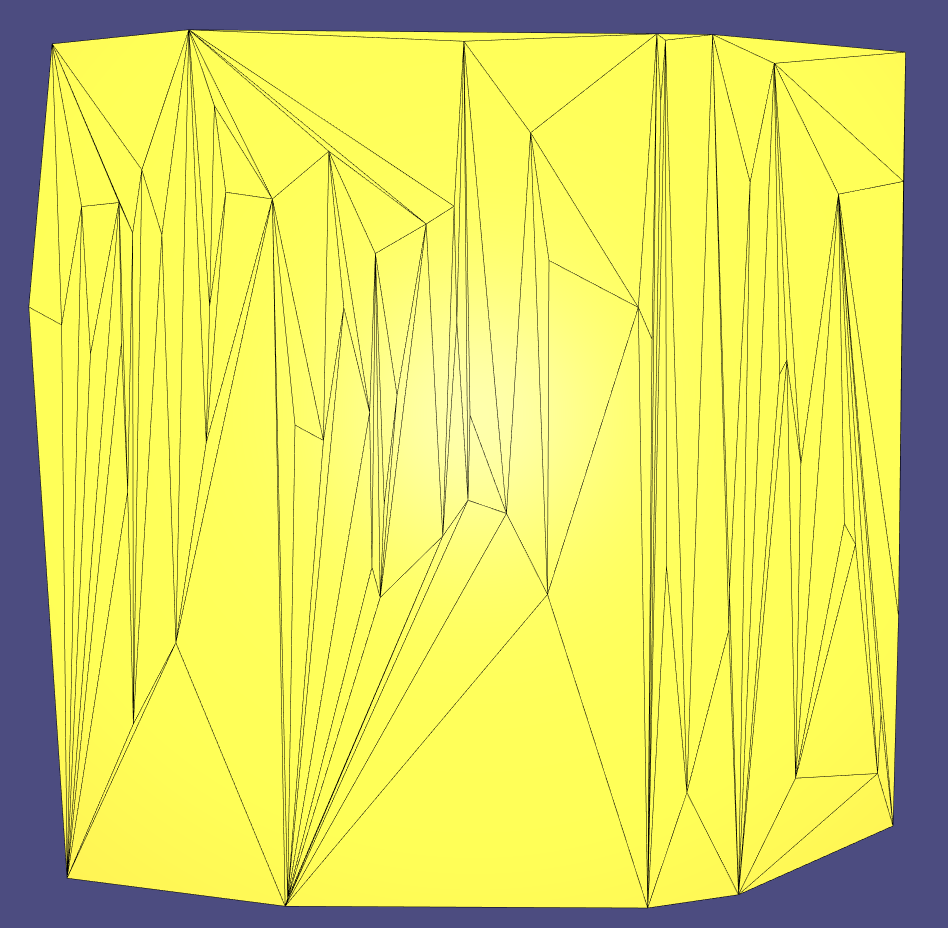
\includegraphics[scale=0.4]{incremental_flat.png}
   		\label{fig:incremental_flat}
    	\caption{Incremental triangulation for 70 points.}
    \end{center}
\end{figure}

\begin{figure}[h]
	\begin{center}
   		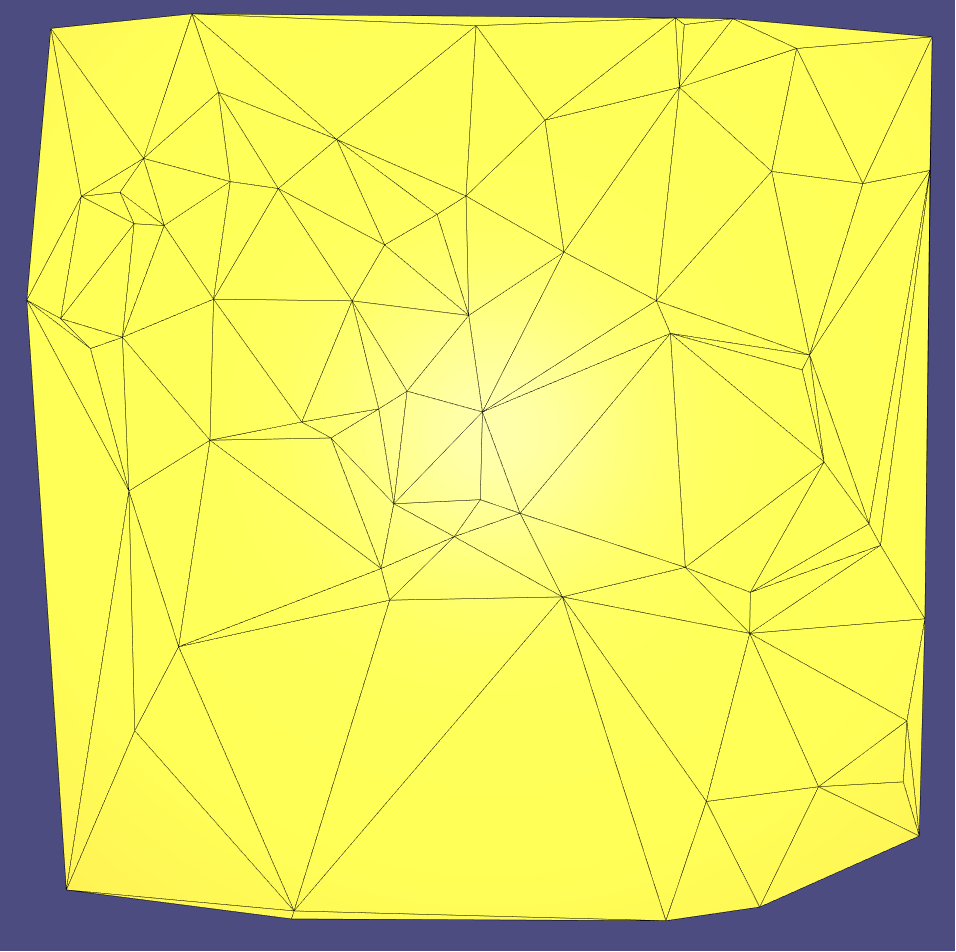
\includegraphics[scale=0.4]{delaunay_flat.png}
    	\caption{A Delaunay triangulation for 70 points, obtained with the Lawson Flip algorithm from the one at Fig. 1.}
    \end{center}
\end{figure}

We present a reconstruction of the height function $2 \dot \sin(x) \dot \cos(y)$ using both the incremental triangulation and a Delaunay triangulation with 500 points.
Note how the incremental triangulation leads to a very bad reconstruction: the skinny and long edges end up producing sharp crests and valleys.
Honestly, the reconstruction almost looks random.
In contrast, the Delaunay leads to a much better reconstruction, resulting in a much smoother surface.
Naturally, we can achieve even better reconstruction by considering more points.
We present a reconstruction using the Delaunay triangulation computed for 2000 sampled points on the $[-20,20]^2$ square.
Note the improvement on the surface reconstruction when compared to using only 500 points.
The respective figures are presented on the next page.

\textit{Obs}: the image files have also been sent along with the other files of this exercise, should you want to see them in greater resolution.

\begin{thebibliography}{99}

\bibitem{dcg}
S. T. Devadoss, J. O'Rouke.
\textit{Discrete and Computational Geometry}, 
Princeton University Press, 2011.

\bibitem{cg13}
B. Gartner, M. Hoffmann. 
\textit{Computational Geometry Lecture Notes HS 2013},
ETH Zurich.

\end{thebibliography}

\begin{figure}[h]
	\begin{center}
   		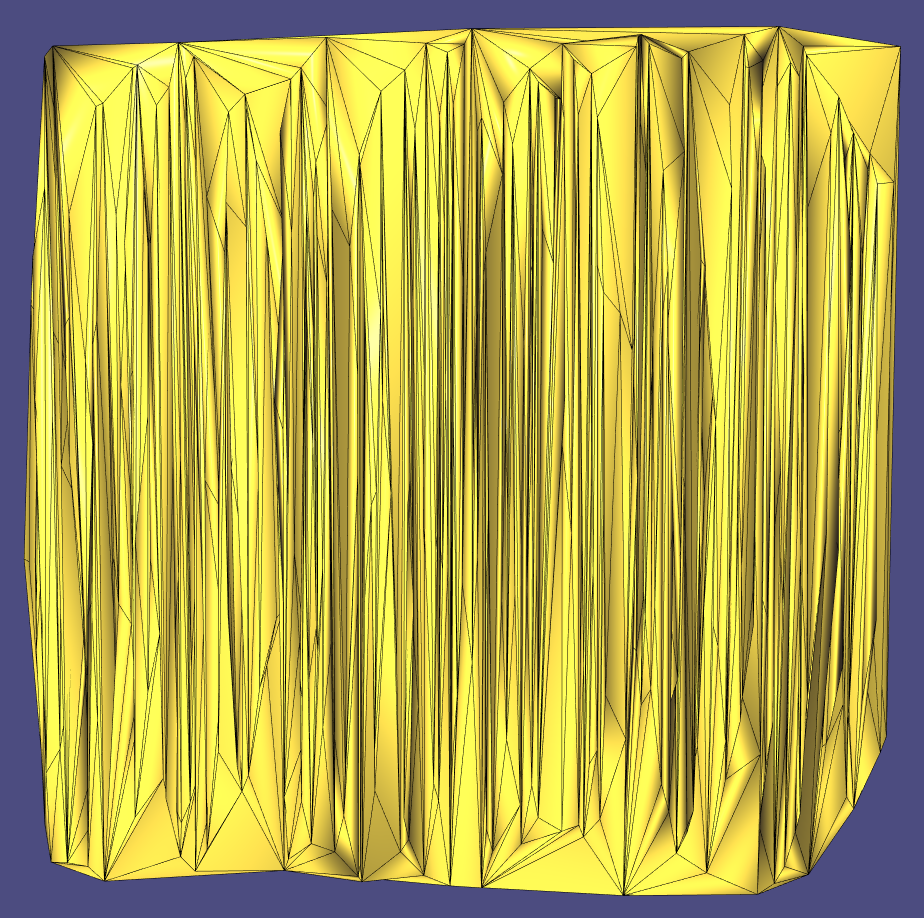
\includegraphics[scale=0.4]{incremental_wavy_500_t1.png}
    	\caption{Surface reconstruction using incremental triangulation with 500 points. Viewed from above.}
    \end{center}
\end{figure}

\begin{figure}[h]
	\begin{center}
   		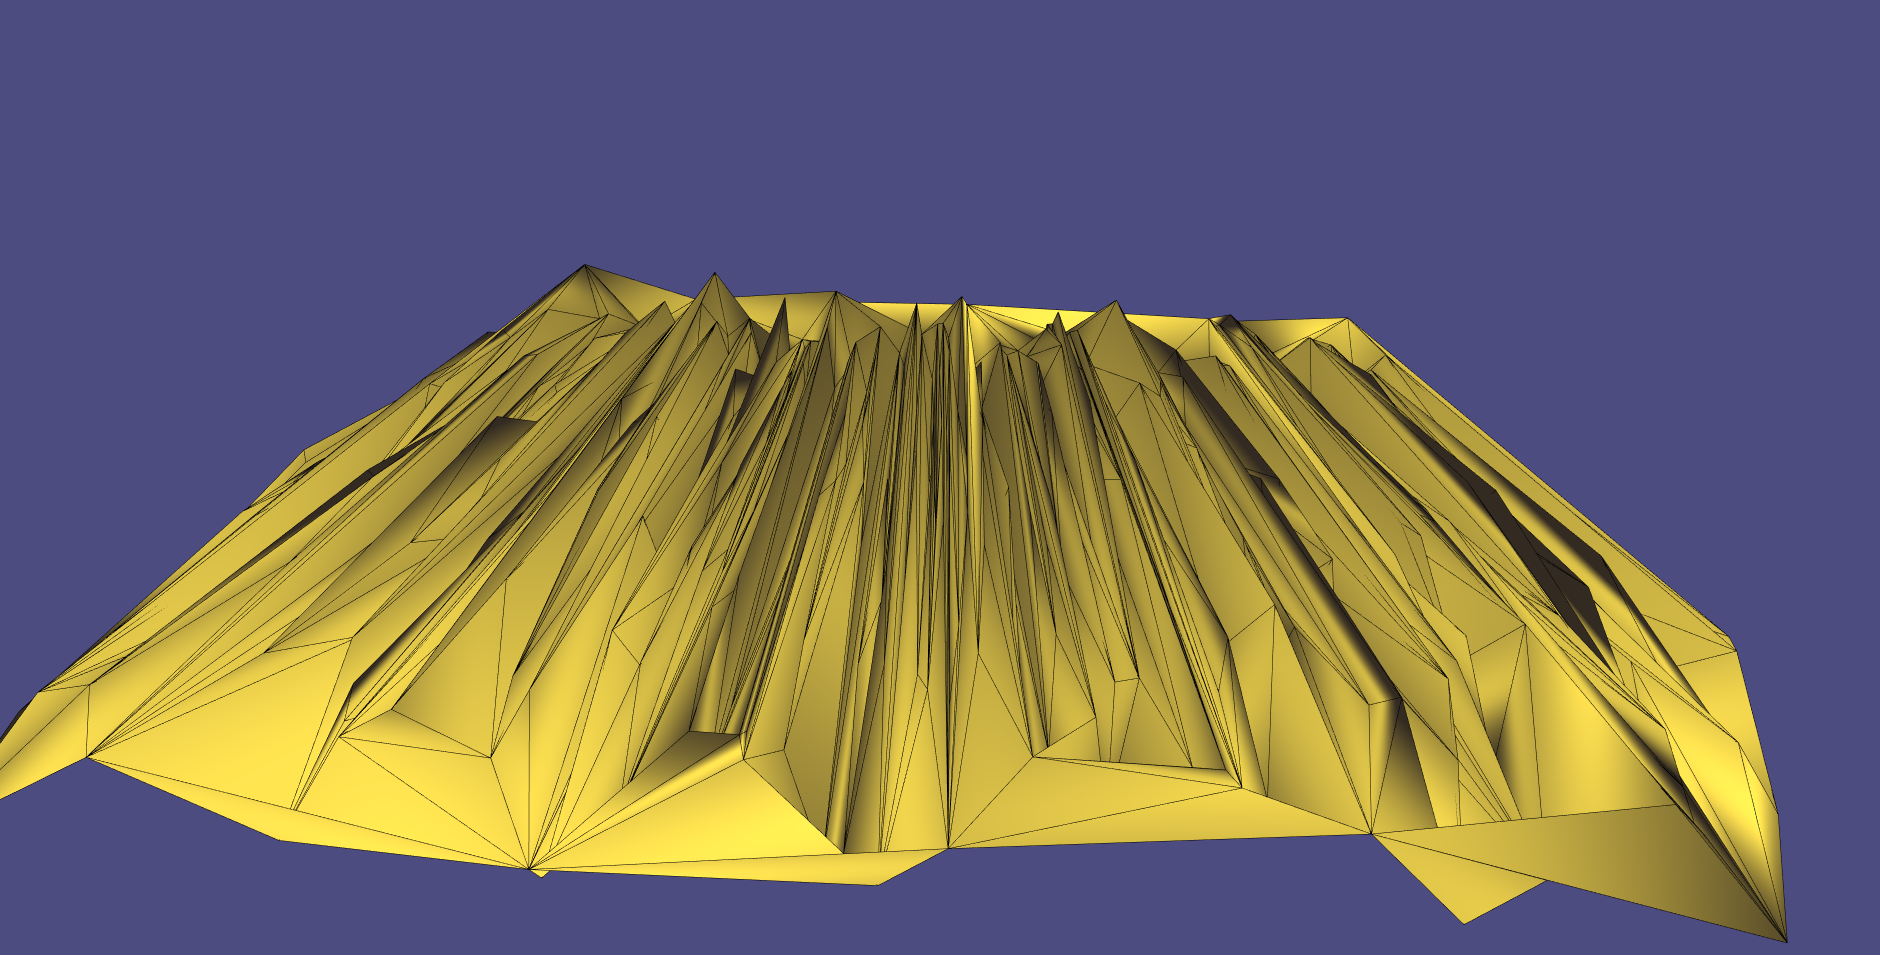
\includegraphics[scale=0.23]{incremental_wavy_500_t2.png}
    	\caption{Surface reconstruction using incremental triangulation with 500 points. Perspective view.}
    \end{center}
\end{figure}

\begin{figure}[h]
	\begin{center}
   		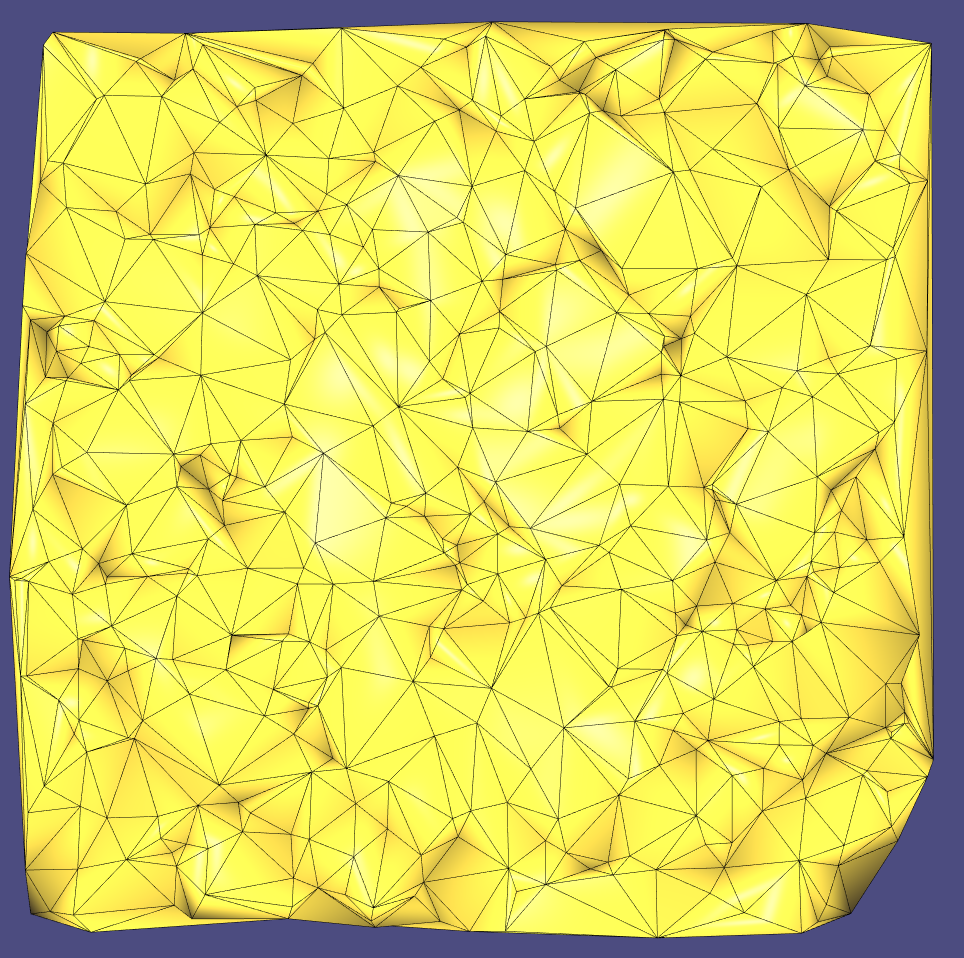
\includegraphics[scale=0.4]{delaunay_wavy_500_t1.png}
    	\caption{Surface reconstruction using a Delaunay triangulation with 500 points. Viewed from above.}
    \end{center}
\end{figure}

\begin{figure}[h]
	\begin{center}
   		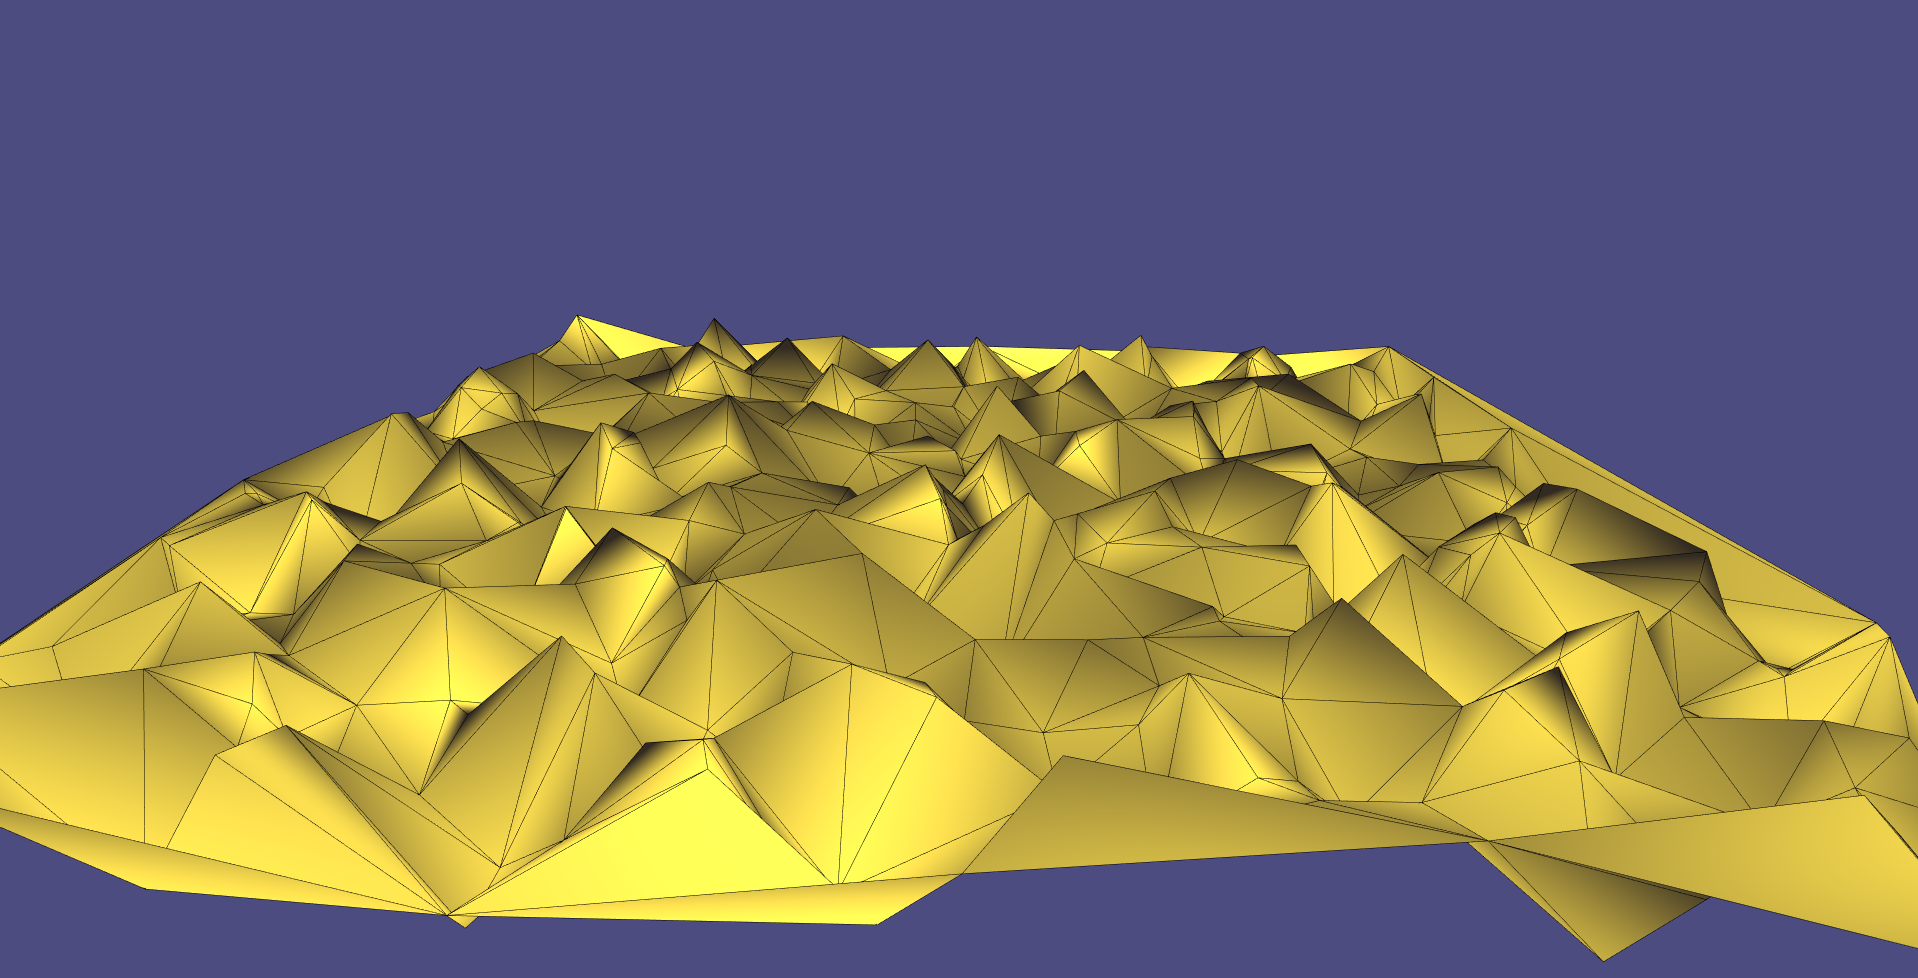
\includegraphics[scale=0.23]{delaunay_wavy_500_t2.png}
    	\caption{Surface reconstruction using a Delaunay triangulation with 500 points. Perspective view.}
    \end{center}
\end{figure}

\begin{figure}[h]
	\begin{center}
   		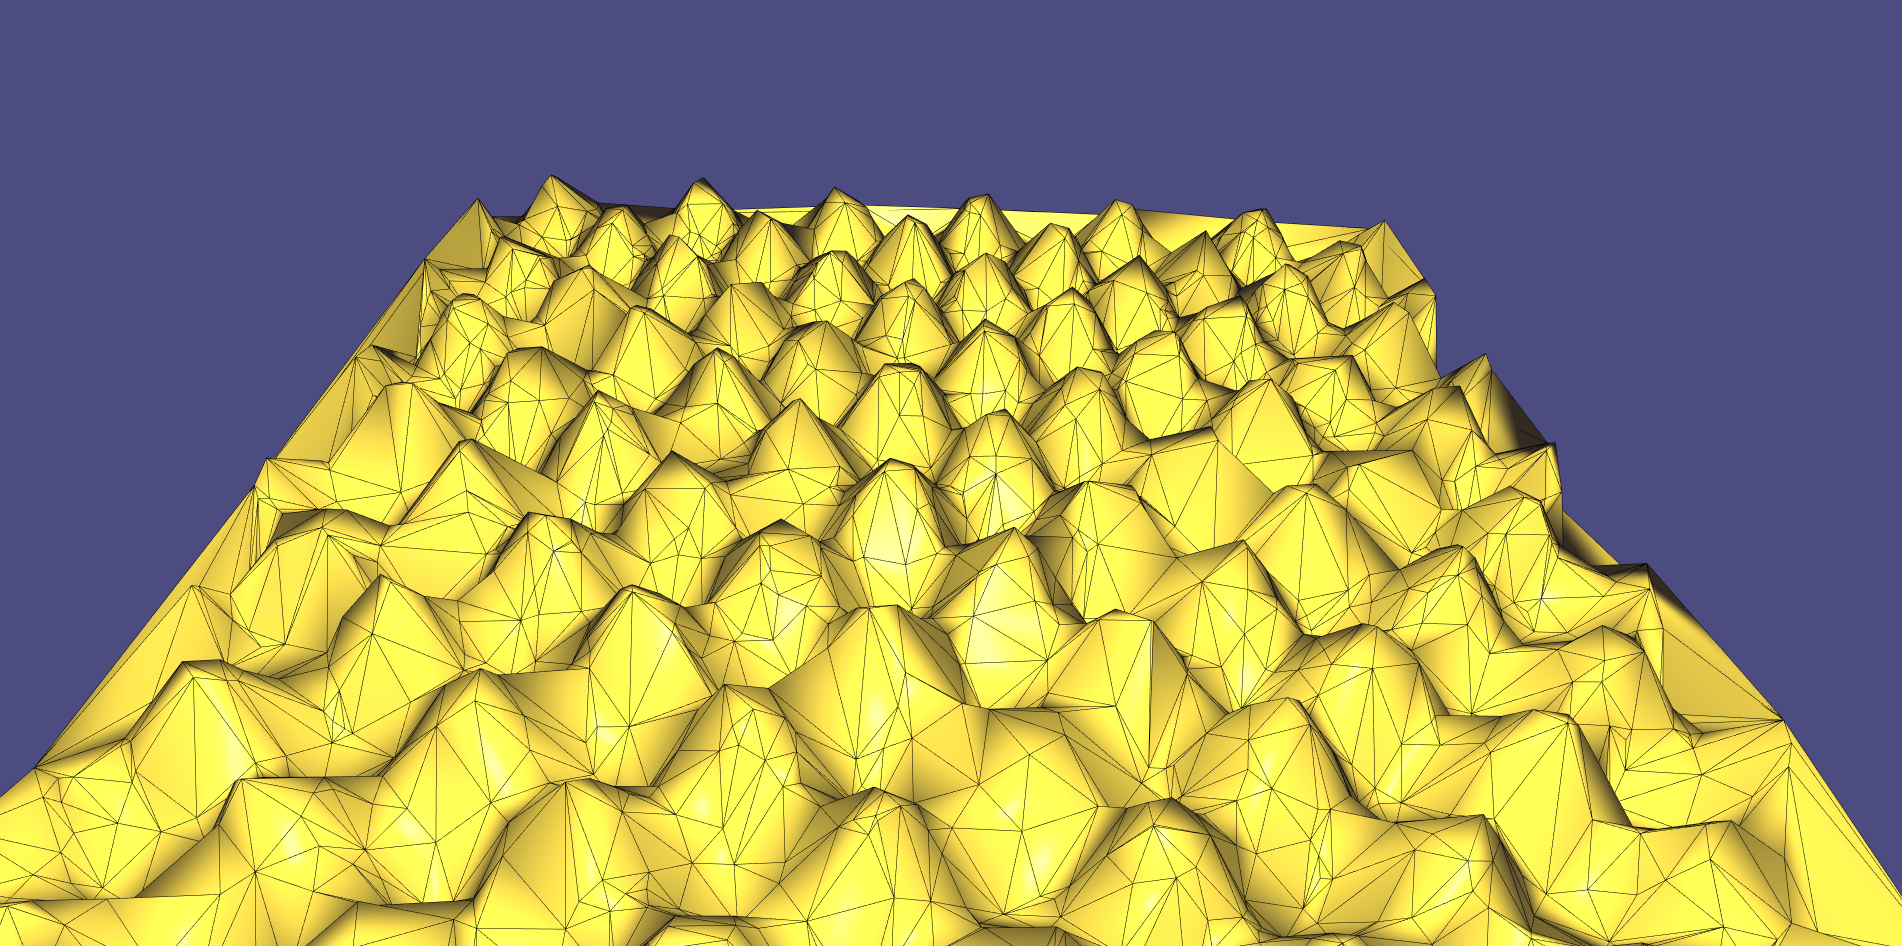
\includegraphics[scale=0.23]{delaunay_wavy_2000_t2.png}
    	\caption{Surface reconstruction using a Delaunay triangulation with 2000 points. Perspective view.}
    \end{center}
\end{figure}

\end{document}